% fig0_executive_summary.tex — Figure 1 (full-width figure*)
% Monochrome executive summary: silent decision -> regulatory gap -> BTV law.
% Regenerated 2026-09-15 (COMSI-2026-04-0112 R1): LGPD Art. 20, moderated
% claim wording, corrected type law direction.
% v2: collision fixes (VLM visual inspection round): stacked regulators in
% band 2 with parallel arrows, label clearances in band 1.
\documentclass[border=2pt]{standalone}
\usepackage{tikz}
\usetikzlibrary{arrows.meta,positioning,fit,calc,shapes.misc}
\usepackage{amssymb}
\usepackage{cmll}
\begin{document}
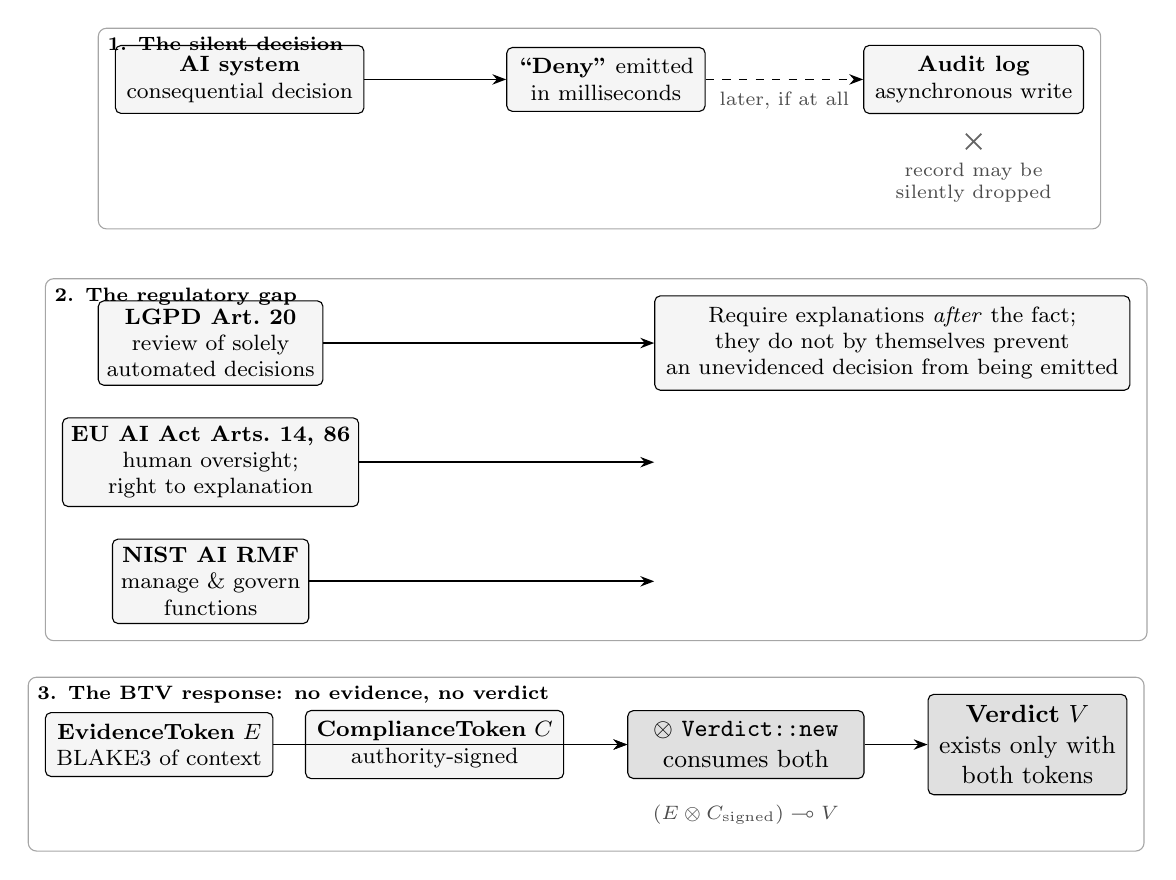
\begin{tikzpicture}[
  font=\footnotesize,
  box/.style={draw, rounded corners=2pt, align=center, inner sep=4pt,
    minimum height=16pt, fill=black!04},
  law/.style={draw, rounded corners=2pt, align=center, inner sep=4pt,
    fill=black!12, font=\small},
  reg/.style={draw, rounded corners=2pt, align=center, inner sep=3pt,
    minimum height=15pt, fill=black!04},
  arr/.style={-{Stealth[length=5pt]}, semithick},
  lost/.style={-{Stealth[length=5pt]}, semithick, dashed},
  note/.style={align=center, font=\scriptsize, text=black!70},
  band/.style={draw=black!35, rounded corners=3pt, inner sep=6pt}
]

% ── Band 1: the silent decision ─────────────────────────────────────────
\node[box] (ai) {\textbf{AI system}\\ consequential decision};
\node[box, right=18mm of ai] (deny) {\textbf{``Deny''} emitted\\ in milliseconds};
\node[box, right=20mm of deny] (log) {\textbf{Audit log}\\ asynchronous write};
\draw[arr] (ai) -- (deny);
\draw[lost] (deny) -- (log)
  node[midway, below=1pt, note] {later, if at all};
\node[draw=black!60, cross out, semithick, below=2.5mm of log, inner sep=2.5pt] (x) {};
\node[note, below=1.5pt of x] (lostlbl) {record may be\\silently dropped};
\node[band, fit=(ai)(deny)(log)(x)(lostlbl), label={[font=\scriptsize\bfseries, anchor=north west]north west:1. The silent decision}] (b1) {};

% ── Band 2: the regulatory gap (stacked regulators, parallel arrows) ────
\node[reg, below=9mm of b1.south west, anchor=north west] (lgpd)
  {\textbf{LGPD Art.~20}\\ review of solely\\automated decisions};
\node[reg, below=4mm of lgpd] (euact)
  {\textbf{EU AI Act Arts.~14,~86}\\ human oversight;\\right to explanation};
\node[reg, below=4mm of euact] (nist)
  {\textbf{NIST AI RMF}\\ manage \& govern\\functions};
\node[box, anchor=west] (gap) at ($(lgpd.east)+(42mm,0)$)
  {Require explanations \emph{after} the fact;\\ they do not by themselves prevent\\
   an unevidenced decision from being emitted};
\draw[arr] (lgpd.east) -- (gap.west |- lgpd);
\draw[arr] (euact.east) -- (gap.west |- euact);
\draw[arr] (nist.east) -- (gap.west |- nist);
\node[band, fit=(lgpd)(euact)(nist)(gap), label={[font=\scriptsize\bfseries, anchor=north west]north west:2. The regulatory gap}] (b2) {};

% ── Band 3: the BTV response ────────────────────────────────────────────
\node[box, below=9mm of b2.south west, anchor=north west, minimum width=20mm] (ev)
  {\textbf{EvidenceToken} $E$\\ BLAKE3 of context};
\node[box, right=4mm of ev, minimum width=20mm] (ct)
  {\textbf{ComplianceToken} $C$\\ authority-signed};
\node[law, right=8mm of ct, minimum width=30mm] (vnew)
  {$\otimes$ \texttt{Verdict::new}\\ consumes both};
\node[law, right=8mm of vnew, minimum width=22mm] (vv)
  {\textbf{Verdict} $V$\\ exists only with\\ both tokens};
\draw[arr] (ev) -- (vnew);
\draw[arr] (ct) -- (vnew);
\draw[arr] (vnew) -- (vv);
\node[note, below=2mm of vnew] (lawnote)
  {$(E \otimes C_{\mathrm{signed}}) \multimap V$};
\node[band, fit=(ev)(ct)(vnew)(vv)(lawnote), label={[font=\scriptsize\bfseries, anchor=north west]north west:3. The BTV response: no evidence, no verdict}] (b3) {};

\end{tikzpicture}
\end{document}
